\documentclass[addpoints]{exam}
% leqno 將方程式編號放在左側

%\printanswers

\usepackage[top=2.5cm,bottom=2cm,left=2.5cm,right=2.5cm,headsep=10pt,a4paper]{geometry} % 引用頁面幾何套件,設定頁面邊界

\usepackage{siunitx} % 角度
% \input{NewCommands}

\usepackage{amsmath,amssymb,amsthm} % 引用常見的數學符號與設定

\usepackage{tikz} 
\usetikzlibrary{arrows.meta}
\usepackage{pgfplots}
\pgfplotsset{compat=1.17}
\usepackage{subcaption}
\usepackage{caption}
\usepackage{xcolor}


\theoremstyle{definition}
\newtheorem*{definition*}{Definition}
\newtheorem*{theorem}{Theorem}
\newtheorem*{remark}{Remark}
\newtheorem*{claim}{Claim}
\newtheorem*{proposition}{Proposition
}
\usepackage{lastpage} % 取得最後頁碼




\usepackage{graphicx} % 引用圖檔內嵌入套件
\graphicspath{{Pictures/}} % 設定圖檔目錄
\usepackage{xcolor} %引用顏色套件
\usepackage{enumerate}
\usepackage{float}
\usepackage{hyperref}
\usepackage{mdwlist} % use suspend & resume to successive enumerate

\usepackage{CJKutf8} % 設定中文

\def \lflr{\left\lfloor} %自定義 floor function
\def \rflr{\right\rfloor} %自定義

% question separation
\renewcommand{\questionshook}{%
  \setlength{\itemsep}{0.5cm}%
}

\allowdisplaybreaks %equation allowed to next page

\firstpageheader{}
                {}
                {}
\footer{}{\sf Page \thepage~of~\pageref{LastPage}}{}

\begin{document}

\begin{CJK*}{UTF8}{gbsn}
% Title
\begin{center}
   {\Large{\bf Introduction to Mathematical Analysis\\
    Homework 11 Due  December  5  (Friday), 2025\\
    Please submit your homework online in PDF format.
  %  Homework X Brief Solution
  }} \\ 
    \large
    %\text{Due date: 3/9/2023}
\end{center}

\noindent\rule{16.2cm}{0.4pt}


\begin{questions}


% ============ Question x ============
\question (20 pts) \textbf{Exercise 5.2.6}  
Let $f \in C(\mathbb{R}/\mathbb{Z}, \mathbb{C})$, and let $(f_n)_{n=1}^\infty$ be a sequence of functions in 
$C(\mathbb{R}/\mathbb{Z}; \mathbb{C})$.

\begin{enumerate}[(a)]
    \item Show that if $f_n$ converges uniformly to $f$, then $f_n$ also converges to $f$ in the $L^2$ metric.

    \item Give an example where $f_n$ converges to $f$ in the $L^2$ metric, but does \emph{not} converge to $f$ uniformly.
    \\
    \emph{(Hint: take $f = 0$. Try to make the functions $f_n$ large in sup norm.)}

    \item Give an example where $f_n$ converges to $f$ in the $L^2$ metric, but does \emph{not} converge to $f$ pointwise.
    \\
    \emph{(Hint: take $f = 0$. Try to make the functions $f_n$ large at one point.)}

    \item Give an example where $f_n$ converges to $f$ pointwise, but does \emph{not} converge to $f$ in the $L^2$ metric.
    \\
    \emph{(Hint: take $f = 0$. Try to make the functions $f_n$ large in $L^2$ norm.)}
\end{enumerate}
\begin{solution}


\end{solution}

\question (20 pts)
Let $\{\phi_N\} : \mathbb{R} \to \mathbb{R}$ be a sequence of continuous, 
periodic functions on $\mathbb{R}$ (with period 1) which satisfy
\[
\int_0^{1} \phi_N(t)\,dt = 1
\qquad\text{and}\qquad
\int_0^{1} |\phi_N(t)|\,dt \le M < \infty
\]
for all $N \in \mathbb{N}$, and
\[
\lim_{N\to\infty} \int_{\delta}^{1 - \delta} |\phi_N(t)|\,dt = 0
\]
for each $0 < \delta < 1$.  

Suppose that $f : \mathbb{R} \to \mathbb{R}$ is continuous and periodic with period $1$.  
Prove that
\[
\lim_{N\to\infty} \int_0^{1} f(x - t)\,\phi_N(t)\,dt = f(x)
\]
uniformly for $x \in \mathbb{R}$.
\begin{solution}


\end{solution}



\question (15 pts)
\noindent\textbf{Exercise 5.2.3.}
If $f \in C(\mathbb{R}/\mathbb{Z};\mathbb{C})$ is a non-zero function,
show that 
\[
0 < \|f\|_{2} \;\le\; \|f\|_{\infty}.
\]

\noindent
Conversely, if $0 < A \le B$ are real numbers, show that there exists a non-zero
function $f \in C(\mathbb{R}/\mathbb{Z};\mathbb{C})$ such that 
\[
\|f\|_2 = A 
\qquad\text{and}\qquad
\|f\|_{\infty} = B.
\]

\noindent
\textit{(Hint: let $g$ be a non-constant non-negative real-valued function in 
$C(\mathbb{R}/\mathbb{Z};\mathbb{C})$, and consider functions of the form
$f=(c + d g)^{1/2}$ for some constant real numbers $c,d>0$.)}
\begin{solution}



\end{solution}


  \question (15 pts)
A \emph{square wave function} is a $\mathbb{Z}$-periodic function defined by
\[
f(x) =
\begin{cases}
1, & x \in [k,\, k + \tfrac{1}{2}),\\[4pt]
-1, & x \in [k + \tfrac{1}{2},\, k + 1),
\end{cases}
\qquad k \in \mathbb{Z}.
\]
Thus $f$ alternates between $1$ and $-1$ on each half-interval, repeating the same
pattern on every interval of length $1$.

Find a sequence of continuous periodic functions which converges in $L^2$ to the
square wave function.

\bigskip

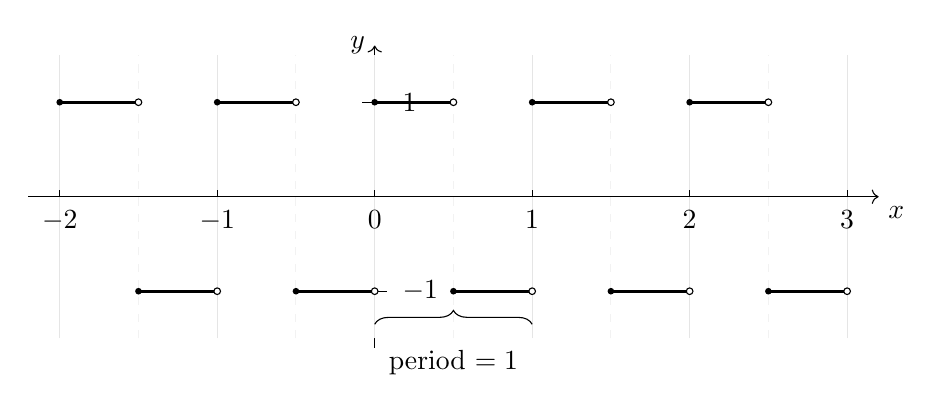
\begin{tikzpicture}[x=2cm,y=1.2cm]

% axes
\draw[->] (-2.2,0) -- (3.2,0) node[below right] {$x$};
\draw[->] (0,-1.6) -- (0,1.6) node[left] {$y$};

% y-level labels
\draw (-0.08,1) -- (0.08,1) node[right=2pt] {$1$};
\draw (-0.08,-1) -- (0.08,-1) node[right=2pt] {$-1$};

% vertical grid at integers and half-integers (light helpers)
\foreach \k in {-2,-1,0,1,2,3}{
  \draw[gray!20] (\k,-1.5) -- (\k,1.5);
}
\foreach \k in {-1.5,-0.5,0.5,1.5,2.5}{
  \draw[gray!10,dashed] (\k,-1.5) -- (\k,1.5);
}

% integer tick labels
\foreach \k in {-2,-1,0,1,2,3}{
  \draw (\k,0) -- (\k,0.07) node[below=4pt] {$\k$};
}

% the square wave: draw for n = -2,...,2
\foreach \n in {-2,-1,0,1,2}{
  % top half: [n, n+1/2) -> y=1
  \draw[line width=1pt] (\n,1) -- (\n+0.5,1);
  % bottom half: [n+1/2, n+1) -> y=-1
  \draw[line width=1pt] (\n+0.5,-1) -- (\n+1,-1);

  % endpoints: closed at left, open at right for each half-interval
  % top half endpoints
  \fill (\n,1) circle (1.2pt); % closed at left
  \draw[fill=white] (\n+0.5,1) circle (1.2pt); % open at right
  % bottom half endpoints
  \fill (\n+0.5,-1) circle (1.2pt); % closed at left
  \draw[fill=white] (\n+1,-1) circle (1.2pt); % open at right
}

% legend for one period
\draw[decorate,decoration={brace,amplitude=5pt}] (0,-1.35) -- (1,-1.35)
  node[midway,below=6pt] {period $=1$};

% labels for pieces
%\node[above right] at (-1.8,1) {$f(x)=1$ on $[n,n+\tfrac12)$};
%\node[below right] at (-1.8,-1) {$f(x)=-1$ on $[n+\tfrac12,n+1)$};

\end{tikzpicture}
  

 


  \question (15 pts)
  
(a) Evaluate 
\[
S_n(\theta) = \sum_{k=1}^{n} \sin(k\theta).
\]

(b) Show that 
\[
|S_n(\theta)| \le \pi \varepsilon^{-1}
\qquad \text{on } [\varepsilon,\, 2\pi - \varepsilon] \text{ for all } n \ge 1.
\]
\begin{solution}


\end{solution}

 \question  (15 pts) Let $f, g \in C(\mathbb{R}/\mathbb{Z}; \mathbb{R})$.  
We define their \emph{periodic convolution} $f * g : \mathbb{R} \to \mathbb{R}$ by
$$
(f * g)(x) := \int_{0}^{1} f(y)\, g(x-y)\, dy.
$$ Prove that $(f * g)$  is smooth whenever $f$ is smooth.
(Remark: A function is called smooth if it has derivatives of all orders.)
\begin{solution}


\end{solution}





\end{questions}


% \appendix
% \section{}
\end{CJK*}
\end{document}

